\documentclass[letterpaper,final,12pt,reqno]{amsart}

\usepackage[total={6.3in,9.2in},top=1.1in,left=1.1in]{geometry}

\usepackage{empheq}
\usepackage[dvipsnames]{xcolor}
\usepackage{graphicx}
\usepackage{verbatim,fancyvrb}
\usepackage{tikz}
\usetikzlibrary{arrows}

% hyperref should be the last package we load
\usepackage[pdftex,
colorlinks=true,
plainpages=false, % only if colorlinks=true
linkcolor=blue,   % only if colorlinks=true
citecolor=Red,   % only if colorlinks=true
urlcolor=black     % only if colorlinks=true
]{hyperref}

\renewcommand{\baselinestretch}{1.05}

\newcommand{\ddt}[1]{\ensuremath{\frac{\partial #1}{\partial t}}}
\newcommand{\ddx}[1]{\ensuremath{\frac{\partial #1}{\partial x}}}
\newcommand{\ddy}[1]{\ensuremath{\frac{\partial #1}{\partial y}}}
\newcommand{\pp}[2]{\ensuremath{\frac{\partial #1}{\partial #2}}}
\renewcommand{\t}[1]{\texttt{#1}}
\newcommand{\Matlab}{\textsc{Matlab}\xspace}
\newcommand{\eps}{\epsilon}
\newcommand{\RR}{\mathbb{R}}

\newcommand{\grad}{\nabla}
\newcommand{\Div}{\nabla\cdot}
\newcommand{\trace}{\operatorname{tr}}


\newcommand{\hbn}{\hat{\mathbf{n}}}

\newcommand{\bg}{\mathbf{g}}
\newcommand{\bn}{\mathbf{n}}
\newcommand{\bu}{\mathbf{u}}
\newcommand{\bv}{\mathbf{v}}

\newcommand{\bX}{\mathbf{X}}



\begin{document}
\graphicspath{{figures/}}

\title[Appendix A]{Appendix A: A finite element Stokes solver \\ for glacier flow}

\author{Ed Bueler}

\maketitle

\vspace{-8mm}
\begin{center}
\footnotesize
\emph{\today}
\end{center}

\thispagestyle{empty}
\bigskip

\renewcommand{\theequation}{A\arabic{equation}}

This is an appendix to my notes \emph{Numerical modelling of glaciers, ice sheets, and ice shelves}---here called ``the notes''---for the International Summer School in Glaciology in McCarthy, Alaska.

We start by stating the Stokes model for ice flow with glacier-suitable boundary conditions.  Next, the specific slab-on-a-slope case is solved exactly, both for verification purposes and so as to give boundary conditions for general cases.  We then derive the ``weak form'' of the Stokes problem.  A brief overview of finite element (FE) methods \cite{Elmanetal2014}, which are based on weak forms, follows.  Our particular FE method uses an unstructured mesh of triangular elements on an arbitrary planar region.  The Stokes problem is solved by a stable ``mixed element'' method with different approximating spaces for velocity and pressure.  Finally we describe a moving-mesh scheme to solve the surface kinematical equation.

The main goal is a numerical velocity and pressure solution, with surface evolution, for a 2D glacier with general geometry, for example with steps in the bedrock (Figure \ref{fig:stepflowlin}).  This numerical model is in short Python codes, as documented at the end, which exploit four advanced open source tools/libraries:
\begin{itemize}
\item Firedrake, an FE library \hfill \url{https://www.firedrakeproject.org/}
\item PETSc, a solver library \hfill \url{http://www.mcs.anl.gov/petsc/}
\item Gmsh, a mesh generator \hfill \url{http://gmsh.info/}
\item Paraview, a visualization tool \hfill \url{https://www.paraview.org/}
\end{itemize}

\begin{figure}[h]
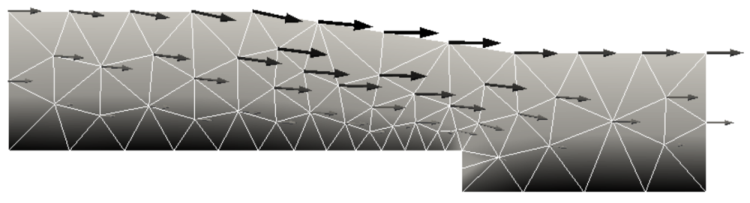
\includegraphics[width=\textwidth,angle=-5.7296]{stepflowlin}  % 0.1 radian = 5.7296 degrees
\caption{A 2D glacier flowing over bedrock steps.  Arrows show velocity $\bu$.  Shading is by pressure $p$.}
\label{fig:stepflowlin}
\end{figure}


\section{Stokes problem}

Recall the Glen-Stokes model in equations (3), (4), (5) from the notes; the model is also described in \cite{GreveBlatter2009,JouvetRappaz2011}.  It applies on a 3D or 2D domain $\Omega$ which must have a smooth-enough boundary to apply the boundary conditions but is otherwise general.  Allowing any Glen exponent $n\ge 1$, the equations are:
\begin{align}
\nabla \cdot \bu &= 0 &&\text{\emph{incompressibility}} \label{incompressible} \\
- \nabla \cdot \tau + \nabla p &= \rho \bg &&\text{\emph{stress balance}} \label{forcebalance} \\
D\bu &= A_n |\tau|^{n-1} \tau &&\text{\emph{Glen flow law}} \label{flowlaw}
\end{align}
The velocity $\bu$, pressure $p$, ice density $\rho$, acceleration of gravity $\bg$, deviatoric stress tensor $\tau$ and strain rate tensor $D\bu$ all appear; recall $D\bu$ involves derivatives of velocity:
\begin{equation}
(D\bu)_{ij} = \frac{1}{2} \left((u_i)_{x_j} + (u_j)_{x_i}\right) \label{strainrate}
\end{equation}

Though the notation here generally follows Table 1 in the notes, some usage is more general or flexible.  For example, the ice softness $A_n$ in \eqref{flowlaw} is now $n$-dependent.  Table 1 shows $A = A_3 = 10^{-16} \,\text{Pa}^{-3}\,\text{a}^{-1} = 3.1689 \times 10^{-24} \,\text{Pa}^{-3}\,\text{s}^{-1}$, but generally the units of $A_n$ are $\text{Pa}^{-n}\,\text{s}^{-1}$.  Regarding tensor norm notation we have:
\begin{align*}
|\tau|^2 = \frac{1}{2} \trace\left(\tau^2\right) = \frac{1}{2} \tau_{ij} \tau_{ij}, \qquad |D\bu|^2 = \frac{1}{2} \trace\left((D\bu)^2\right) = \frac{1}{2} (D\bu)_{ij} (D\bu)_{ij}
\end{align*}

Tensors $D\bu$ and $\tau$ are symmetric and have trace zero.  The full (Cauchy) stress tensor $\sigma$ is the deviatoric stress tensor $\tau$ minus the pressure,
\begin{equation}
    \sigma = \tau - p\,I,  \label{cauchystress}
\end{equation}
so equation \eqref{forcebalance} is simply $-\Div \sigma = \rho \bg$.  One may derive from \eqref{cauchystress} that $p = -\frac{1}{3} \trace(\sigma)$ in 3D, thus that the pressure is the negative of the average normal stress.  By definition $\Div\tau$ in \eqref{forcebalance} is a vector with components which are the divergences of the rows:
\begin{equation}
    \left(\nabla \cdot \tau\right)_i = \left(\tau_{i1}\right)_{x_1} + \left(\tau_{i2}\right)_{x_2} + \left(\tau_{i3}\right)_{x_3}  \label{divtaudefn}
\end{equation}
Thus $\nabla\cdot \tau$ is a column vector like $\nabla p$ and $\bg$ in \eqref{forcebalance}.

Recall the viscosity form of \eqref{flowlaw}, namely equation (15) in the notes:
\begin{equation}
\tau = 2\nu D\bu = B_n |D\bu|^{\frac{1}{n} - 1} D\bu  \label{viscflowlaw}
\end{equation}
Here $B_n = (A_n)^{-1/n}$ is the $n$-dependent ice hardness in units $\text{Pa}\,\text{s}^{1/n}$.  From \eqref{viscflowlaw} we can eliminate $\tau$ from equations \eqref{forcebalance}, \eqref{flowlaw} and rewrite them in terms of velocity and pressure only:
\begin{align}
\Div \bu &= 0 \label{incompagain} \\
- \nabla \cdot \left(B_n |D\bu|^{\frac{1}{n} - 1} D\bu\right) + \nabla p &= \rho \mathbf{g} \label{stokes}
\end{align}
The Stokes model is, from now on, equations \eqref{incompagain}, \eqref{stokes} with certain boundary conditions.  The solution is the velocity-pressure pair $(\bu,p)$.

Certain glacier-suitable velocity and stress boundary conditions are used in our example.  To explain these, consider the numerical solution shown in Figure \ref{fig:stepflowlin}.  We assume that the base, top, inflow, and outflow boundary surfaces can all be identified.  On the base we require no slip:
\begin{align}
\bu &= 0  &&\text{\emph{base}} \label{basebc} \\
\intertext{On the top we set a condition of zero applied stress, $\sigma\hbn=0$ or equivalently:}
\left(B_n |D\bu|^{\frac{1}{n} - 1} D\bu - pI\right) \hbn &= 0  &&\text{\emph{top}} \label{topbc} \\
\intertext{The left-side inflow boundary has outward normal $\hbn=\left<-1,0,0\right>^\top$ in all cases we solve.  On this surface we set a nonzero inflow velocity:}
\bu &= \left<f(z),0,0\right>^\top  &&\text{\emph{inflow}} \label{inflowbc} \\
\intertext{The inflow $f(z)$ will satisfy the slab-on-slope equations for a specific thickness $H_{\text{in}}$ at the inflow; see below.  On the outflow boundary, where $\hbn=\left<1,0,0\right>^\top$, $h$ is the surface elevation, and $g=|\bg|$, we set a nonzero hydrostatic normal stress and zero traction:}
\left(B_n |D\bu|^{\frac{1}{n} - 1} D\bu - pI\right) \hbn &= C_{\text{out}} \left<- \rho g \cos\alpha (h-z),0, \rho g\sin\alpha (h-z)\right>^\top  &&\text{\emph{outflow}} \label{outflowbc}
\end{align}
The constant $C_{\text{out}} $ is adjusted so that the total applied stress is equal to its value for ice thicknesses $H_{\text{in}}$: $C_{\text{out}} = (H_{\text{in}}/H_{\text{out}})^2$ where $H_{\text{out}}$ is the varying outflow ice thickness.


\section{Slab-on-slope solutions}

Testing a numerical model requires verification tools, namely exact solutions.  Thus we recapitulate the construction of slab-on-slope solutions, as given in the notes, this time allowing any Glen exponent $n$.  We also determine the $n$-dependent ice hardness $B_n$ so that these solutions have the same surface velocity for any $n$, and construct the inflow and outflow boundary conditions based on based on the slab-on-slope case.

Suppose the domain $\Omega$ is 2D, namely points $(x,y,z)$ where $y=0$.  Denote the components of velocity as $\bu=\left<u,v,w\right>$.  Suppose there is no variation in the cross-flow direction ($\partial/\partial y=0$) and no cross-flow velocity ($v=0$).  Also assume the force of gravity is downward but at angle $\alpha$ with the $z$-direction so $\bg = \left<g\sin\alpha,0,-g\cos\alpha\right>$ where $g=|\bg|$.  Equations \eqref{incompagain}, \eqref{stokes} now become the system
\begin{align}
u_x + w_z &= 0 \label{planeincomp} \\
- \left(B_n |D\bu|^{\frac{1}{n}-1} u_x\right)_x - \left(B_n |D\bu|^{\frac{1}{n}-1} \frac{1}{2} \left(u_z+w_x\right)\right)_z + p_x &= \rho g\sin\alpha \label{planestressx} \\
- \left(B_n |D\bu|^{\frac{1}{n}-1} \frac{1}{2} \left(u_z+w_x\right)\right)_x - \left(B_n |D\bu|^{\frac{1}{n}-1} w_z\right)_z + p_z &= -\rho g\cos\alpha \label{planestressz}
\end{align}
The strain-rate norm expands/simplifies to
\begin{equation}
    |D\bu| = \sqrt{\frac{1}{2} \left(u_x^2 + \frac{1}{2}(u_z+w_x)^2 + w_z^2\right)}  \label{planeDnorm}
\end{equation}
Equations \eqref{planeincomp}--\eqref{planeDnorm} are the 2D (strong) form of the Stokes model, written-out using coordinates $(x,z)$ and velocity $\bu=\left<u,w\right>$.

Now suppose there is no variation in $x$, i.e.~that $\partial/\partial_x=0$, and that the domain $\Omega$ is a slab such that $b < z < h$ for fixed ($x$-independent) values of the bed elevation $b$ and the surface elevation $h$.  This is the situation of an infinitely-long (or periodic) slab flow with $x$-independent boundary stresses (e.g.~no lubricated spots at the base).  Then the system simplifies to $w_z=0$ and
\begin{equation}
- \left(B_n |D\bu|^{\frac{1}{n}-1} \frac{1}{2} u_z\right)_z = \rho g\sin\alpha, \quad
- \left(B_n |D\bu|^{\frac{1}{n}-1} w_z\right)_z + p_z = -\rho g\cos\alpha \label{slabstresses}
\end{equation}
The strain-rate norm simplifies to $|D\bu| = \sqrt{\frac{1}{2} \left(\frac{1}{2}u_z^2 + w_z^2\right)}$.

If we further assume that there is no slip at the base then $w=0$ identically.  Then the second of equations \eqref{slabstresses} allows integration with respect to $z$ yielding a formula for $p$.  Assuming zero pressure at the surface gives the hydrostatic pressure profile
\begin{equation}
p(z) = \rho g\cos\alpha (h-z)  \label{pslab}
\end{equation}
Also $|D\bu| = \frac{1}{2} |u_z|$.  From \eqref{slabstresses} we now have a single nontrivial equation to solve for the horizontal velocity:
    $$- \left(\frac{B_n}{2^{\gamma+1}} |u_z|^\gamma u_z\right)_z = \rho g\sin\alpha$$
The flow of a viscous, non-sliding fluid on a uniform slab will be such that $u_z>0$, so, with rearrangement, the equation is now
    $$\left((u_z)^{1/n} \right)_z = - \frac{2^{1/n} \rho g\sin\alpha}{B_n}$$
Again this can be integrated from the surface $z=h$, using the no-stress (no traction) condition, which simplifies to $u_z=0$, to give
\begin{equation}
u_z = 2 \left(\frac{\rho g\sin\alpha}{B_n}\right)^n (h-z)^n  \label{uzslab}
\end{equation}
Integrating vertically one more time, from the base $z=b$ where $u=0$, gives
\begin{equation}
u(z) = \frac{2}{n+1} \left(\frac{\rho g\sin\alpha}{B_n}\right)^n \left((h-b)^{n+1} - (h-z)^{n+1}\right)  \label{uslab}
\end{equation}

Suppose we want comparable solutions, with glaciologically-reasonable ice velocities, for any $n\ge 1$.  Ice sheet modeling tradition \cite{GreveBlatter2009}, and glaciological experiments starting with Glen, suggest we base our work on $n=3$.  From the ice softness value $A_3 = 3.1689 \times 10^{-24} \,\text{Pa}^{-3}\,\text{s}^{-1}$ we get $B_3 = (A_3)^{-1/3} = 6.8082\times 10^7\,\text{Pa}\,\text{s}^{1/3}$.  We now compute $B_n$ for any $n\ge 1$ such the slab-on-slope surface velocity $u(h)$ from \eqref{uslab} matches the value in the $n=3$ case.  The result is
\begin{equation}
B_n = \left(\frac{4}{n+1}\right)^{1/n} \Big(\rho g \sin\alpha (h-b)\Big)^{(n-3)/n} {B_3\,}^{3/n}  \label{Bnfromsurface}
\end{equation}
For example, suppose $h-b=400$ m and $\alpha=0.1$ radians (about $5.7$ degrees).  Using $B_n$ from \eqref{Bnfromsurface} gives a surface velocity of $u(h)=906.092 \,\text{m}\,\text{a}^{-1}$ from \eqref{uslab} independent of $n\ge 1$.  For some glaciologically-relevant end-cases $n=1,4$ \cite{GoldsbyKohlstedt2001}, the result from \eqref{Bnfromsurface} is $B_1=4.9663\times 10^{12}\,\text{Pa}\,\text{s}$ and $B_4=1.7320\times 10^{7}\,\text{Pa}\,\text{s}^{1/4}$.  The Newtonian viscosity $\nu=B_1/2$ is about $10^{16}$ times more viscous than liquid water but about $10^7$ times less viscous than granite (both at $25^\circ \,\text{C}$, and according to wikipedia).

Formulas \eqref{pslab} and \eqref{uslab} will be used for verifying the numerical solver.  Additionally they allow us to set boundary conditions which lead to glaciologically-reasonable solutions even when modeling a small part of a glacier.  Specifically we do this for the geometry shown in Figure \ref{fig:stepflowlin}.  The inflow side of the region has \eqref{uslab} applied as a Dirichlet condition, i.e.~equation \eqref{inflowbc}.  Also, the outflow side has a normal stress computed from the slab-on-slope solution.  From \eqref{uzslab} above, and the facts that $w=0$, $u_x=0$, and $|D\bu| = \frac{1}{2} u_z$, we find that because $\hbn=\left<1,0\right>$ is the outward normal on the outflow side,
\begin{align*}
\sigma \hbn &= \left(B_n |D\bu|^{\frac{1}{n}-1} D\bu - pI\right)\hbn = \left(B_n |D\bu|^{\frac{1}{n}-1} \begin{pmatrix} u_x & \frac{1}{2}(u_z+w_x) \\ \frac{1}{2}(u_z+w_x) & w_z \end{pmatrix} - pI\right)\hbn \\
    &= B_n \left(\frac{1}{2} u_z\right)^{\frac{1}{n}-1} \begin{pmatrix} 0 \\ \frac{1}{2} u_z \end{pmatrix} - \begin{pmatrix} p \\ 0 \end{pmatrix} = \begin{pmatrix} - p \\ \frac{B_n}{2^{1/n}} (u_z)^{1/n} \end{pmatrix} = \begin{pmatrix} - \rho g\cos\alpha (h-z) \\ \rho g\sin\alpha (h-z) \end{pmatrix}
\end{align*}
This justifies formula \eqref{outflowbc}.


\section{Weak form}

The Stokes equations \eqref{incompagain}, \eqref{stokes} are PDEs called the \emph{strong form} of the model.  An integral equation form of the same model, called the \emph{weak form}, is needed to construct an FE method \cite{Elmanetal2014}.  It is derived by multiplying the strong form equations by \emph{test functions} and then integrating over $\Omega$ so as to define a scalar-valued nonlinear functional $F$ (formula \eqref{defineF} below).  The weak form says that $F$ must be zero when acting on test functions.

The significance of the weak form is two-fold:
\begin{itemize}
\item It has a larger space of potential solutions than the strong form and thus it is more flexible with respect to discontinuities in the data.  It is well-posed in the sense of having a unique solution  for a wide range of boundary values \cite{JouvetRappaz2011}.
\item The FE method generates weak form test functions by local constructions which work on any triangular mesh.  Such constructions are more flexible with respect to mesh geometry than are finite difference methods based on the strong form.
\end{itemize}
The latter of these points, namely that the FE method can be adapted to unstructured meshes, is of greater practical importance.

The solution to the weak form is the pair $(\bu,p)$ where $\bu\in V_D$ and $p \in Q$ for function spaces (\emph{trial functions}) precisely identified in \cite{JouvetRappaz2011}.  Test functions come from nearly the same spaces: $(\bv,q)$ with $\bv\in V_0$ and $q\in Q$.  The difference in the velocity space relates only to the Dirichlet boundary conditions; $\bu\in V_D$ satisfies base and inflow boundary conditions (namely, equations \eqref{basebc} and \eqref{inflowbc}) while $\bv\in V_0$ is zero on those boundaries.

We multiply \eqref{incompagain} by $q\in Q$ and \eqref{stokes} by $\bv\in V_0$, then add and integrate to define $F$:
\begin{equation}
F(\bu,p;\bv,q) = \int_\Omega - \left(\nabla \cdot \left(B_n |D\bu|^{\frac{1}{n} - 1} D\bu\right)\right)\cdot \bv + \nabla p \cdot \bv - \rho \mathbf{g} \cdot \bv - \left(\nabla \cdot \bu\right) q \label{nonfuncone}
\end{equation}
Next, integration-by-parts rewrites $F$ to balance the number of derivatives on $(\bv,q)$ and $(\bu,p)$.  For this step, recall the product rule $\nabla \cdot(f\bX) = \grad f\cdot \bX + f \nabla \cdot \bX$ and the divergence theorem $\int_\Omega \nabla \cdot \bX = \int_{\partial \Omega} \bX \cdot \hbn$.  Again denoting $\tau = B_n |D\bu|^{\frac{1}{n} - 1} D\bu$, we have
\begin{align*}
\int_\Omega \left(\nabla \cdot \tau\right)\cdot \bv &= \sum_{j=1}^3 \int_\Omega \nabla \cdot (\tau_{j\circ})\, v_j = \sum_{j=1}^3 \int_\Omega \nabla \cdot (\tau_{j\circ} v_j) - \tau_{j\circ} \nabla v_j \\
  &= \sum_{j=1}^3 \int_{\partial \Omega} (\tau_{j\circ} v_j) \cdot \hbn - \int_\Omega \tau_{j\circ} \cdot \nabla v_j = \int_{\partial \Omega} (\tau \hbn)\cdot \bv - \int_\Omega \trace(\tau \nabla \bv)
\end{align*}
where $\circ$ denotes a vector entry index and $\tau_{j\circ}$ denotes the $j$th row of $\tau$.  Here $\grad\bv$ defines a $3\times 3$ matrix,
\newcommand{\trefthree}[3]{\left[\begin{array}{c|c|c} & & \\ #1 & #2 & #3 \\ & & \end{array}\right]}
    $$\grad \bv = \trefthree{\grad v_1}{\grad v_2}{\grad v_3} = \begin{bmatrix}
    (v_1)_{x_1} & (v_2)_{x_1} & (v_3)_{x_1} \\
    (v_1)_{x_2} & (v_2)_{x_2} & (v_3)_{x_2} \\
    (v_1)_{x_3} & (v_2)_{x_3} & (v_3)_{x_3}
    \end{bmatrix}$$
and so
    $$\trace(\tau \grad \bv) = \sum_{j=1}^3 \tau_{j\circ} \cdot \grad v_j = \sum_{i,j=1}^3 \tau_{ji} (v_j)_{x_i}$$
Some sources \cite{JouvetRappaz2011} write $A:B$ for $\trace(AB)$.  Note $\trace(\tau \grad \bv) = \trace(\tau D\bv)$ because $\trace(AB)=0$ if $A$ is symmetric and $B$ is antisymmetric.  (To show this take $A=\tau$ and $B=\grad\bv-D\bv$.)  Finally we do a straightforward integration-by-parts on the pressure part of $F$:
    $$\int_\Omega \nabla p \cdot \bv = \int_\Omega \nabla\cdot (p\,\bv) - p (\nabla \cdot \bv) = \int_{\partial \Omega} p\hbn \cdot \bv - \int_\Omega p (\nabla \cdot \bv)$$

The above facts allow us to rewrite \eqref{nonfuncone} with a normal stress boundary integral:
\begin{equation}
F(\bu,p;\bv,q) = -\int_{\partial\Omega} (\sigma \hbn)\cdot \bv + \int_\Omega \trace(\tau D\bv) - p (\nabla \cdot \bv) - \left(\nabla \cdot \bu\right) q - \rho \mathbf{g} \cdot \bv \label{nonfunctwo}
\end{equation}
(We have denoted $\sigma=\tau-pI$ for brevity.)  Now $\bu,\bv$ appear with at most first derivatives and $p,q$ appear without derivatives.

Recall that $\bv\in V_0$ satisfies $\bv=0$ along the base and inflow surfaces so these parts of the integral over $\partial\Omega$ in \eqref{nonfunctwo} are zero.  Conditions \eqref{topbc}, \eqref{outflowbc} therefore completely eliminate the unknown solution $\bu,p$ from the boundary integral.  This yields our final formula for the nonlinear functional:
\begin{align}
F(\bu,p;\bv,q) &= \int_\Omega B_n |D\bu|^{\frac{1}{n} - 1} \trace(D\bu D\bv) - p (\nabla \cdot \bv) - \left(\nabla \cdot \bu\right) q \label{defineF} \\
    &\qquad  - \int_\Omega \rho \mathbf{g} \cdot \bv - \int_{\{\text{outflow}\}} \rho g (h-z) v_1  \notag
\end{align}
The last two integrals can be regarded as source terms.  For example, if the inflow velocity is zero and if we replace the source terms by zero---no gravity or outflow stress---then the unique solution is $\bu=0$ and $p=0$ \cite{Elmanetal2014}.

The finalized weak formulation of the Stokes model is the statement that, at the solution $\bu\in V_D$ and $p\in Q$, functional $F$ in \eqref{defineF} is zero in all test function directions:
\begin{equation}
F(\bu,p;\bv,q) = 0 \qquad \text{ for all } \bv\in V_0 \text{ and } q\in Q  \label{weak}
\end{equation}
This weak formulation is proven in \cite{JouvetRappaz2011} to be well-posed under reasonable assumptions about the domain $\Omega$ and boundary data.  These assumptions will be satisfied in the cases we consider.  Now our goal is to approximate this one solution pair $(\bu,p)$ numerically.


\section{Finite element method}

This section gives a necessarily very abbreviated summary of the FE method we apply, through calls to Firedrake (see below), to solve the Stokes equations.  More serious coverage of the FE method is in the references \cite{Braess2007,BuelerBook,Elmanetal2014}


\section{Surface kinematical equation}

A glacier may change shape as it flows, and so we want our model to do that too.  Suppose the domain on which the Stokes equations apply is the time-dependent set
\begin{equation}
\Omega^t = \left\{(x,z)\,\big|\, b(x) < z < h(x,t)\right\}  \label{Omegat}
\end{equation}
where $z=b(x)$ is the base elevation and $z=h(x,t)$ is the ice surface elevation.  The base elevation function $b(x)$ is time-independent in our simplified model.  The ice also does not slide \eqref{basebc}, nor melt or refreeze liquid water at the base, and thus the base kinematical (equation (42) in the notes) reduces to ``$0=0$.''  (No effort is needed to solve this equation!)  However, the time-dependent surface $z=h(x,t)$ evolves according to a nontrivial surface kinematical equation ((41) in the notes).  In 2D, where the ice velocity is $\bu=\left<u(x,z,t),w(x,z,t)\right>$, this equation says
\begin{equation}
h_t = a(x,t) - u(x,h,t) h_x + w(x,h,t) \label{surfacekinematical}
\end{equation}

Here $a(x,t)$ is the climatic mass balance in units $\text{m}\,\text{s}^{-1}$.  In our examples below $a=0$, because we study ice fluid dynamics in isolation, but most scientific questions about glaciers require nontrivial models for $a$.  Implementation of nonzero values for $a(x,t)$ is straightforward if done in an explicit or time-split manner; see below.

Equation \eqref{surfacekinematical} applies on a time-dependent 1D domain (curve), the ice surface:
    $$\Gamma^t = \left\{(x,z) \,\big|\, z = h(x,t)\right\}$$
Informally, \eqref{surfacekinematical} determines the change in surface elevation $\Delta h \approx h_t\,\Delta t$ as the climatically added/removed ice $a\,\Delta t$ plus the component of the ice motion in the normal direction $\bn = \left<-h_x,1\right>$, thus $\Delta h \approx a \,\Delta t + \bn\cdot \bu\big|_{z=h} \Delta t$.  However, as pointed-out by \cite[pp.~65--66]{GreveBlatter2009}, the surface $\Gamma^t$ is also the $\Phi=0$ level surface of the function
    $$\Phi(x,z,t) = z - h(x,t)$$
We regard this function as being defined on the closure of $\Omega^t$, including $\Gamma^t$.  Since $\grad \Phi = \left<-h_x,1\right>$ is an outward normal along $\Gamma^t$,
\begin{equation}
h_t = a + (\grad \Phi)\big|_{\Gamma^t} \cdot \bu\big|_{\Gamma^t}  \label{surfacekinematicalwithPhi}
\end{equation}
The advantage of using \eqref{surfacekinematicalwithPhi} over \eqref{surfacekinematical} is that in Firedrake (see below) it is easier to compute the gradient of the current 2D scalar field $\Phi(x,z,t_n)$, and evaluate it along the boundary, than it is to compute the derivative of the current surface elevation $h(x,t_n)$.

We can now describe our explicit time-stepping strategy for modeling a changing glacier.  It solves the surface kinematical equation \eqref{surfacekinematical} or \eqref{surfacekinematicalwithPhi} by vertically-displacing the triangular mesh.  Note that in the FE scheme (see below) the mesh is given by scalar coordinate fields $(x,z)$defined on all the nodes of the mesh.  The current ice surface elevation $z=h(x,t_n)$ can be described as the values of $z$ on the identified top boundary of the current domain/mesh $\Omega^n$.  Given a time step $\Delta t > 0$, the strategy is this iteration:

\medskip
\renewcommand{\labelenumi}{\emph{\arabic{enumi}.}}
\begin{enumerate}
\item Solve the weak-form Stokes equation \eqref{weak} for current values $(\bu^n,p^n)$ at $t=t_n$ on the current mesh $\Omega^n$.
\item From the current mesh $\Omega^n$ generate the current piecewise-linear surface elevation function $h^n(x)$.
\item Evaluate $\Phi^n(x,z) = z - h^n(x)$ on $\Omega^n$, and define the following function on $\Omega^n$:
\begin{equation}
\Delta h^n =  \Delta t\,\left(a(x,t_n) + \grad \Phi^n\cdot \bu^n\right) \label{deltahfield}
\end{equation}
\item Solve the following Dirichlet problem (Laplace equation) for a vertical displacement field $r^n$:
\begin{align}
- \grad^2 r^n &= 0 & &\text{on } \Omega^n \label{vdisplacementpoisson} \\
          r^n &= 0 & &\text{on inflow, base, and outflow parts of } \partial \Omega^n \notag \\
          r^n &= \Delta h^n & &\text{on the top boundary } \Gamma^n \notag
\end{align}
(In fact the problem is solved in weak form, namely $\int_{\Omega^n} \grad r^n\cdot \grad w = 0$ for all test functions $w$ satisfying $w=0$ on the entire boundary $\partial \Omega^n$.)
\item Define a new mesh which has vertical-only displacement by $r^n$:
\begin{equation}
  x^{n+1} = x^n, \quad z^{n+1} = z^n + r^n \label{updatemesh}
\end{equation}
\item Repeat at \emph{1}.
\end{enumerate}

\medskip
At the end of an iteration the new top boundary $\Gamma^{n+1}$ is the surface $z=h^{n+1}(x)$.  By \eqref{deltahfield} an iteration does an explicit step of \eqref{surfacekinematicalwithPhi}:
    $$h^{n+1}(x) = h^n(x) + \Delta t\,\left(a(x,t_n) + \grad \Phi^n\cdot \bu^n\right)$$
The significance of Dirichlet problem \eqref{vdisplacementpoisson} is that the entire mesh is \emph{smoothly} displaced, in the vertical direction only by \eqref{updatemesh}, because solutions of the Laplace equation, which minimize $\int |\grad r|^2$ over functions with the given boundary values, are smooth.

Note that the scheme uses fixed time step $\Delta t > 0$ and is explicit.  At best the strategy is conditionally stable, and in practice that is observed.  It should be expected that, as with an SIA solver, the time step is restricted by a condition like ``$D\Delta t / \Delta x^2 < 1$'' where $\Delta x$ is a representative mesh spacing variable and $D$ is some diffusivity parameter meaningful in the current context.  However, there is presently no theory in the literature which describes $D$ or otherwise supplies a sufficient stability restriction.  The extensive testing needed to develope a practical time-step restriction has barely been started.


\section{Implementation in Python codes}

We implement the above numerical approach in Python codes which directly import the Firedrake FE library, and indirectly the PETSc solver library as well.  An example time-independent run looks like this:

\medskip
\begin{Verbatim}
$ ./gendomain.py -o glacier.geo                # creates domain outline
$ gmsh -2 glacier.geo                          # meshes domain
$ source ~/firedrake/bin/activate              # starts Firedrake
(firedrake) $ ./flow.py glacier.msh            # solves Stokes problem
(firedrake) $ paraview glacier.pvd             # visualizes results
\end{Verbatim}
%$

\medskip
\noindent In a time-stepping run one also gives the time step in days and the number of steps as arguments to \texttt{flow.py}:

\medskip
\begin{Verbatim}
(firedrake) $ ./flow.py -deltat 20.0 -m 10 glacier.msh
\end{Verbatim}
%$

\medskip
\noindent The Python codes \texttt{gendomain.py} and \texttt{flow.py} also provide command-line help with a \texttt{-h} option.

\medskip
As shown in Figure \ref{blockdiagram} there are two Python codes which the user calls, namely \texttt{gendomain.py} and \texttt{flow.py}, and two additional Python modules imported into \texttt{flow.py}.  These four Python codes perform the following actions:
\begin{itemize}
\item \texttt{flow.py}: \quad  This executable main driver code reads user options, reads the mesh from a Gmsh \texttt{.msh} file, sets-up Firedrake function spaces, either solves a single time-independent Stokes problem or executes the above time-stepping strategy (according to options), and writes the solution for visualization into a Paraview-readable \texttt{.pvd} file.  The solution can also be visualized in a surface-values figure under option \texttt{-osurface}.  Imports functions from each of the following three Python codes.
\item \texttt{gendomain.py}: \quad  An executable code which writes an outline of the initial domain \eqref{Omegat} into an ASCII file (\texttt{.geo} extension) using the Gmsh-readable geometry description language.  Portions of the boundary are marked with integer tags; see the Python dictionary \texttt{bdryids}.  Also defines a function \texttt{getdomaindims()} which can dynamically-extract certain dimensions from a changing mesh.
\item \texttt{meshactions.py}: \quad  This module provides mesh manipulation functions.  The most important  are \texttt{getsurfaceelevationfunction\_halos()}, which extracts a piecewise-linear surface elevation function $h(x)$ from the current mesh, and \texttt{solvevdisp()}.  The latter assembles and solves the Dirichlet problem \eqref{vdisplacementpoisson}, using Firedrake's linear \texttt{solve()} command, and applies the solution as a vertical mesh movement \eqref{updatemesh}.  It sets the option prefix \texttt{vd\_} for PETSc options to control this solver.  There are also other functions used for visualization.
\item \texttt{physics.py}: \quad  Most actual ice physics is isolated in this module, including ice physical constants and the Stokes problem weak form \eqref{defineF}.  The most important function here is \texttt{stokessolve()} which assembles and solves the Stokes problem \eqref{weak} using Firedrake's nonlinear \texttt{solve()} command, and it sets the PETSc solver option prefix \texttt{s\_}.
\end{itemize}

\begin{figure}[h]
\bigskip
\tikzstyle{tool} = [draw, minimum size=2em]
\tikzstyle{other} = [draw, minimum size=2em,rounded corners=0.2cm]
\begin{tikzpicture}[node distance=3.8cm,auto,>=latex']
    \node [tool] (gendomain) {\texttt{gendomain.py}};
    \node [other] (gmsh) [right of= gendomain] {Gmsh};
    \node [tool] (flow) [right of=gmsh] {\texttt{flow.py}};
    \node [other] (paraview) [right of=flow] {Paraview};
    \node [tool,dashed] (physics) [above left of=flow, xshift=1cm, yshift=-0.5cm] {\texttt{physics.py}};
    \node [tool,dashed] (meshactions) [above right of=flow, xshift=-1cm, yshift=-0.5cm] {\texttt{meshactions.py}};
    \path[->] (gendomain) edge node {\texttt{.geo}} (gmsh) ;
    \path[->] (gmsh) edge node {\texttt{.msh}} (flow) ;
    \path[->] (flow) edge node {\texttt{.pvd}} (paraview) ;
    \path[->] (gendomain) edge [dashed, bend left] node {} (flow) ;
    \path[->] (physics) edge [dashed] node {} (flow) ;
    \path[->] (meshactions) edge [dashed] node {} (flow) ;
\end{tikzpicture}
\label{blockdiagram}

\medskip
\caption{The tools are used in the given order (solid), with input/output file formats as shown.  Python module \texttt{import}s are dashed.}
\end{figure}


\small

\bigskip
\bibliography{stokes}
\bibliographystyle{siam}

\end{document}
